\documentclass[a4paper]{arrowhead}

\usepackage[yyyymmdd]{datetime}
\usepackage{etoolbox}
\usepackage[utf8]{inputenc}
\usepackage{multirow}
\usepackage{hyperref}

\renewcommand{\dateseparator}{-}

\setlength{\parskip}{1em}

%% Special references
\newcommand{\fref}[1]{{\textcolor{ArrowheadBlue}{\hyperref[sec:functions:#1]{#1}}}}
\newcommand{\mref}[1]{{\textcolor{ArrowheadPurple}{\hyperref[sec:model:#1]{#1}}}}
\newcommand{\pdef}[1]{{\textcolor{ArrowheadGrey}{#1\label{sec:model:primitives:#1}\label{sec:model:primitives:#1s}\label{sec:model:primitives:#1es}}}}
\newcommand{\pref}[1]{{\textcolor{ArrowheadGrey}{\hyperref[sec:model:primitives:#1]{#1}}}}

\newrobustcmd\fsubsection[3]{
  \addtocounter{subsection}{1}
  \addcontentsline{toc}{subsection}{\protect\numberline{\thesubsection}function \textcolor{ArrowheadBlue}{#1}}
  \renewcommand*{\do}[1]{\rref{##1},\ }
  \subsection*{
    \thesubsection\quad
    operation
    \textcolor{ArrowheadBlue}{#1}
    (\notblank{#2}{\mref{#2}}{})
    \notblank{#3}{: \mref{#3}}{}
  }
  \label{sec:functions:#1}
}
\newrobustcmd\msubsection[2]{
  \addtocounter{subsection}{1}
  \addcontentsline{toc}{subsection}{\protect\numberline{\thesubsection}#1 \textcolor{ArrowheadPurple}{#2}}
  \subsection*{\thesubsection\quad#1 \textcolor{ArrowheadPurple}{#2}}
  \label{sec:model:#2} \label{sec:model:#2s} \label{sec:model:#2es}
}

\begin{document}

%% Arrowhead Document Properties
\ArrowheadTitle{Service Registry Core System}
\ArrowheadType{System Description}
\ArrowheadTypeShort{SysD}
\ArrowheadVersion{4.5.0}
\ArrowheadDate{\today}
\ArrowheadAuthor{Tamás Bordi}
\ArrowheadStatus{RELEASE}
\ArrowheadContact{tbordi@aitia.ai}
\ArrowheadFooter{\href{www.arrowhead.eu}{www.arrowhead.eu}}
\ArrowheadSetup
%%

%% Front Page
\begin{center}
  \vspace*{1cm}
  \huge{\arrowtitle}

  \vspace*{0.2cm}
  \LARGE{\arrowtype}
  \vspace*{1cm}

  %\Large{Service ID: \textit{"\arrowid"}}
  \vspace*{\fill}

  % Front Page Image
  %\includegraphics{figures/TODO}

  \vspace*{1cm}
  \vspace*{\fill}

  % Front Page Abstract
  \begin{abstract}
    This document provides system description for the \textbf{Service Registry Core System}.
  \end{abstract}

  \vspace*{1cm}

%   \scriptsize
%   \begin{tabularx}{\textwidth}{l X}
%     \raisebox{-0.5\height}{
\includegraphics[width=2cm]{figures/artemis_logo}} & {ARTEMIS Innovation Pilot Project: Arrowhead\newline
%     THEME [SP1-JTI-ARTEMIS-2012-AIPP4 SP1-JTI-ARTEMIS-2012-AIPP6]\newline
%     [Production and Energy System Automation Intelligent-Built environment and urban infrastructure for sustainable and friendly cities]}
%   \end{tabularx}
%   \vspace*{-0.2cm}
 \end{center}

\newpage
%%

%% Table of Contents
\tableofcontents
\newpage
%%

\section{Overview}
\label{sec:overview}
\color{black}
This document describes the Service Registry Core System, which exists to enable service discovery within an Eclipse Arrowhead Local Cloud (LC). Examples of such interactions is a provider system offering some kind of service for use by other systems in the LC. This mandatory Core System provides the data storage functionality for the information related to the currently and actively offered Services within the Local Cloud.

The rest of this document is organized as follows.
In Section \ref{sec:prior_art}, we reference major prior art capabilities
of the system.
In Section \ref{sec:use}, we describe the intended usage of the system.
In Section \ref{sec:properties}, we describe fundamental properties
provided by the system.
In Section \ref{sec:delimitations}, we describe delimitations of capabilities
of the system.
In Section \ref{sec:services}, we describe the abstract service
operations produced by the system.
In Section \ref{sec:security}, we describe the security capabilities
of the system.

\newpage

\subsection{Significant Prior Art}
\label{sec:prior_art}

The strong development on cloud technology and various requirements for digitisation and automation has led to the concept of Local Clouds (LC).

\textit{"The concept takes the view that specific geographically local automation tasks should be encapsulated and protected."} \cite{jerker2017localclouds}

One of the main building blocks when realizing such Local Cloud is the capability of storing and maintaining information about the systems and services belonged to the given LC.

\subsection{How This System Is Meant to Be Used}
\label{sec:use}

Service Registry is a mandatory core system of Eclipse Arrowhead LC and is responsible for the fundamental service discovery functionality. Systems and services are being discoverable for other systems by consuming the services provided by Service Registry Core System.

An application or other core system is required to register itself and its services into Service Registry if it is designed to be part of the Local Cloud and to unregister before shutdown or when it does not intend to continue to provide its services.

\subsection{System functionalities and properties}
\label{sec:properties}

\subsubsection {Functional properties of the system}
Service Registry solves the following needs to fulfill the requirements of service discovery.

\begin{itemize}
    \item Enables the application and other core systems to register themselves in order to being part of the Local Cloud.
    \item Enables the application and other core systems to unregister themselves from the Local Cloud.
    \item Enables the application and other core systems to publish their services within the Local Cloud.
    \item Enables the application and other core systems to revoke their services from the Local Cloud.
    \item Makes the offered services queryable for other systems within the Local Cloud.
\end{itemize}

\subsubsection {Non functional properties of the system}
Beside the requirements of service discovery the Service Registry implements certain authentication of systems, meaning that Service Registry makes decision whether a given system has right to join to the Local Cloud or not.

\subsubsection {Data stored by the system}
In order to achieve the mentioned functionalities, Service Registry is capable to store the information set described by figure \ref{fig:information_overview}.

\begin{figure}[h!]
  \centering
  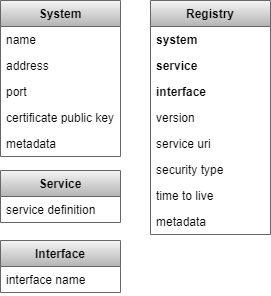
\includegraphics[width=8cm]{figures/serviceregistry_data_overview.png}
  \caption{
    Overview of data stored by Service Registry Core System.
  }
  \label{fig:information_overview}
\end{figure}

\subsection{Important Delimitations}
\label{sec:delimitations}

While Service Registry Core System is responsible to decide who can join to the Local Cloud, it is not responsible to decide that which system is authorized to consume which service, therefore only the so called \textit{"public core services"} are allowed to query directly from Service Registry.

Querying \textit{"not public"} services directly from Service Registry is primarily permitted to Orchestrator Mandatory Core System, while maintaining authorization rules between systems and services is the responsibility of Authorization Mandatory Core System.

\newpage

\section{Services produced}
\label{sec:services}

\msubsection{service}{echo}
The purpose of this service is to test the system availability. The service is offered for both application and core systems. 

\msubsection{service}{service-register}
The purpose of this service is to publish the provided services and make them discoverable. The service is offered for both application and core systems. 

\msubsection{service}{service-unregister}
The purpose of this service is to revoke the published services. The service is offered for both application and core systems. 

\msubsection{service}{register-system}
The purpose of this service is to join to the Local Cloud. The service is offered for both application and core systems.

\msubsection{service}{unregister-system}
The purpose of this service is to leave the Local Cloud. The service is offered for both application and core systems.

\msubsection{service}{query}
The purpose of this service is to look-up possible provider systems for one specific service. The service is offered for both application and core systems.

\msubsection{service}{query-multi}
The purpose of this service is to look-up possible provider systems for a set of service. The service is offered only for specified core systems.

\msubsection{service}{query-all}
The purpose of this service is to return all the currently active service instance. The service is offered only for specified core systems.

\msubsection{service}{query-by-system}
The purpose of this service is to return the exact system record by system name, address and port. The service is offered only for specified core systems.

\msubsection{service}{query-by-system-id}
The purpose of this service is to return the exact system record by the record id. The service is offered only for specified core systems.

\msubsection{service}{pull-system}
The purpose of this service is to return all system registered into the Local Cloud. The service is offered only for specified core systems.

\newpage

\section{Security}
\label{sec:security}

The security of Eclipse Arrowhead - and therefore the security of Service Registry  - is relying on X.509 certificate trust chains. The Arrowhead trust chain consists of three level:
\begin{itemize}
    \item Master certificate: \texttt{arrowhead.eu}
    \item Cloud certificate: \texttt {my-cloud.my-company.arrowhead.eu}
    \item Client certificate: \texttt{my-client.my-cloud.my-company.arrowhead.eu}
\end{itemize}

For Arrowhead certificate profile see \url{https://github.com/eclipse-arrowhead/documentation}

\bibliographystyle{IEEEtran}
\bibliography{bibliography}

\newpage

\section{Revision History}
\subsection{Amendments}

\noindent\begin{tabularx}{\textwidth}{| p{1cm} | p{3cm} | p{2cm} | X | p{4cm} |} \hline
\rowcolor{gray!33} No. & Date & Version & Subject of Amendments & Author \\ \hline

1 & YYYY-MM-DD & \arrowversion & & Xxx Yyy \\ \hline
\end{tabularx}

\subsection{Quality Assurance}

\noindent\begin{tabularx}{\textwidth}{| p{1cm} | p{3cm} | p{2cm} | X |} \hline
\rowcolor{gray!33} No. & Date & Version & Approved by \\ \hline

1 & YYYY-MM-DD & \arrowversion  &  \\ \hline

\end{tabularx}

\end{document}